i\documentclass[tikz,border=3mm]{standalone}
\usepackage[T1]{fontenc}
\usepackage{helvet}                       % IEEE-recommended Helvetica
\renewcommand{\familydefault}{\sfdefault}
\usepackage{amsmath,amssymb}
\usepackage{tikz}
\usetikzlibrary{shapes.geometric, positioning, decorations.pathreplacing,
                arrows.meta, calc}

\begin{document}
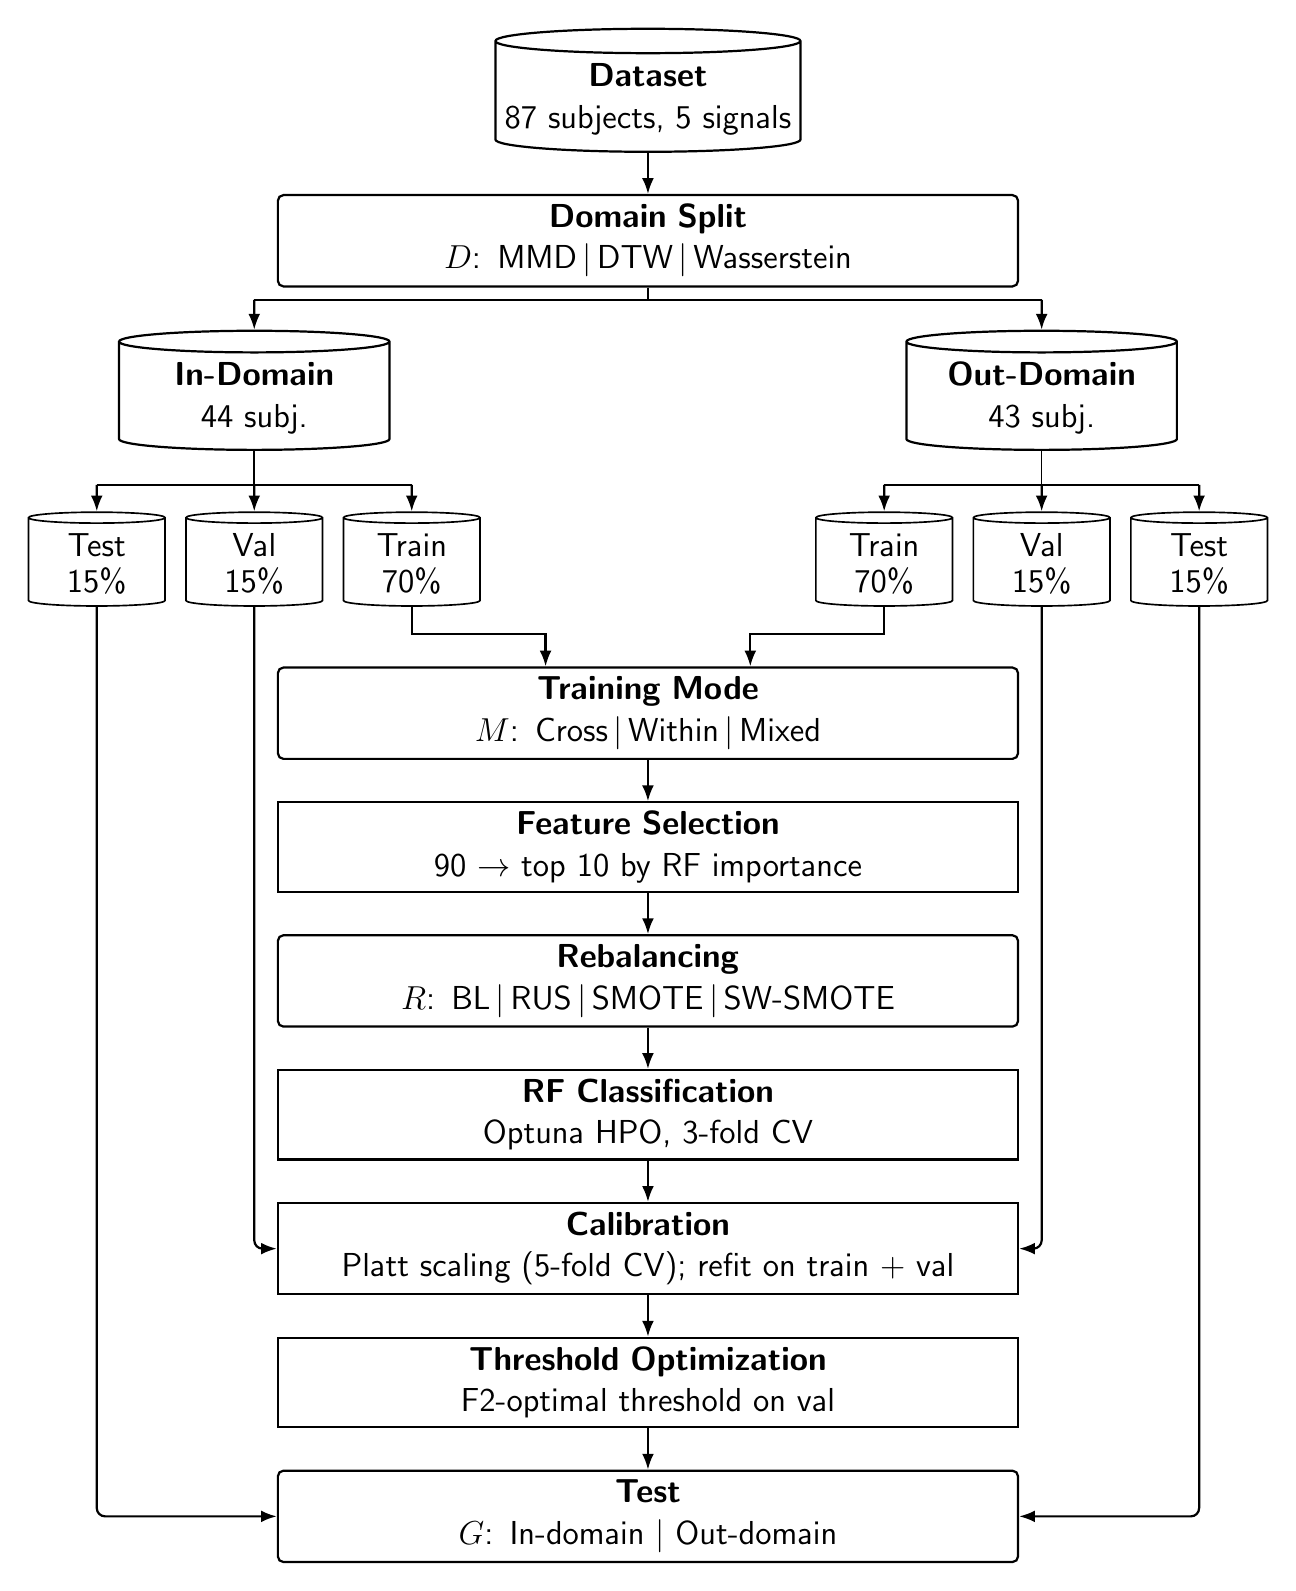
\begin{tikzpicture}[
  % ---- Base font: 8pt Helvetica → ~9–10pt when printed at IEEE column width ----
  every node/.style={font=\sffamily\large},
  >=Latex,
  % ---- Node styles ----
  db/.style={draw, thick, cylinder, cylinder uses custom fill,
    cylinder body fill=white, shape border rotate=90, aspect=0.08,
    minimum width=3.4cm, minimum height=1.0cm, align=center,
    font=\sffamily\large},
  dbsm/.style={draw, semithick, cylinder, cylinder uses custom fill,
    cylinder body fill=white, shape border rotate=90, aspect=0.08,
    minimum width=1.7cm, minimum height=0.75cm, text width=1.5cm,
    align=center, font=\sffamily\large},
  % Experimental-factor box (rounded corners, light gray)
  fbox/.style={draw, thick, rounded corners=2pt,
    text width=9.0cm, minimum width=9.4cm,
    minimum height=0.7cm, align=center, fill=white,
    font=\sffamily\large},
  % Processing-step box (sharp corners, white)
  pbox/.style={draw, thick,
    text width=9.0cm, minimum width=9.4cm,
    minimum height=0.7cm, align=center, fill=white,
    font=\sffamily\large},
  % ---- Arrow styles (distinguishable in greyscale) ----
  arr/.style ={-{Latex[length=2mm, width=1.5mm]}, thick},
  darr/.style={-{Latex[length=2mm, width=1.5mm]}, semithick, dashed},           % validation
  dtarr/.style={-{Latex[length=2mm, width=1.5mm]}, semithick, densely dotted},  % test
  % ---- Annotation font (consistent secondary size) ----
  annot/.style={font=\sffamily\large},
]

%%% ============================================================
%%% ROW 0 — Dataset
%%% ============================================================
\node[db] (dataset) at (0,0)
  {\textbf{Dataset}\\[1pt]
   87 subjects, 5 signals};

%%% ============================================================
%%% ROW 1 — Domain Split  (factor D)
%%% ============================================================
\node[fbox] (dsplit) at (0,-1.8)
  {\textbf{Domain Split}\\[1pt]
   $D$: MMD\,$|$\,DTW\,$|$\,Wasserstein};
\draw[arr] (dataset.south) -- (dsplit.north);

%%% ============================================================
%%% ROW 2 — In-Domain / Out-Domain  (factor G)
%%% ============================================================
\node[db, text width=3.2cm] (src) at (-5.0,-3.8)
  {\textbf{In-Domain}\\[1pt] 44 subj.};
\node[db, text width=3.2cm] (tgt) at ( 5.0,-3.8)
  {\textbf{Out-Domain}\\[1pt] 43 subj.};

\coordinate (forkTop) at (0,-2.55);
\draw[thick] (dsplit.south) -- (forkTop);
\draw[thick] (-5.0,-2.55) -- (5.0,-2.55);
\draw[arr]   (-5.0,-2.55) -- (src.north);
\draw[arr]   ( 5.0,-2.55) -- (tgt.north);

%%% ============================================================
%%% ROW 3 — Subject-level temporal split  (70 / 15 / 15)
%%% ============================================================
% Source side: Test (outer) — Val — Train (inner)
\node[dbsm] (test_s)  at (-7.0,-5.9)
  {Test\\[-1pt] 15\%};
\node[dbsm] (val_s)   at (-5.0,-5.9)
  {Val\\[-1pt] 15\%};
\node[dbsm] (train_s) at (-3.0,-5.9)
  {Train\\[-1pt] 70\%};

\coordinate (forkS) at (-5.0,-4.9);
\draw[semithick] (src.south) -- (forkS);
\draw[semithick] (-7.0,-4.9) -- (-3.0,-4.9);
\draw[arr] (-7.0,-4.9) -- (test_s.north);
\draw[arr] (-5.0,-4.9) -- (val_s.north);
\draw[arr] (-3.0,-4.9) -- (train_s.north);

% Target side: Train (inner) — Val — Test (outer)
\node[dbsm] (train_t) at (3.0,-5.9)
  {Train\\[-1pt] 70\%};
\node[dbsm] (val_t)   at (5.0,-5.9)
  {Val\\[-1pt] 15\%};
\node[dbsm] (test_t)  at (7.0,-5.9)
  {Test\\[-1pt] 15\%};

\coordinate (forkT) at (5.0,-4.9);
\draw[semithick] (tgt.south) -- (forkT);
\draw[semithick] (3.0,-4.9) -- (7.0,-4.9);
\draw[arr] (3.0,-4.9) -- (train_t.north);
\draw[arr] (5.0,-4.9) -- (val_t.north);
\draw[arr] (7.0,-4.9) -- (test_t.north);

%%% ============================================================
%%% ROW 4 — Training Mode  (factor M)
%%% ============================================================
\node[fbox] (mode) at (0,-7.8)
  {\textbf{Training Mode}\\[1pt]
   $M$: Cross\,$|$\,Within\,$|$\,Mixed};

\draw[arr] (train_s.south) -- ++(0,-0.35) -| ([xshift=-1.3cm]mode.north);
\draw[arr] (train_t.south) -- ++(0,-0.35) -| ([xshift= 1.3cm]mode.north);

%%% ============================================================
%%% ROW 5 — Feature Selection
%%% ============================================================
\node[pbox] (fs) at (0,-9.5)
  {\textbf{Feature Selection}\\[1pt]
   90 $\to$ top 10 by RF importance};
\draw[arr] (mode.south) -- (fs.north);

%%% ============================================================
%%% ROW 6 — Rebalancing  (factor R)
%%% ============================================================
\node[fbox] (reb) at (0,-11.2)
  {\textbf{Rebalancing}\\[1pt]
   $R$: BL\,$|$\,RUS\,$|$\,SMOTE\,$|$\,SW-SMOTE};
\draw[arr] (fs.south) -- (reb.north);

%%% ============================================================
%%% ROW 7 — RF Classification  (Optuna HPO)
%%% ============================================================
\node[pbox] (cls) at (0,-12.9)
  {\textbf{RF Classification}\\[1pt]
   Optuna HPO, 3-fold CV};
\draw[arr] (reb.south) -- (cls.north);

%%% ============================================================
%%% ROW 8 — Calibration  (refit on train + val)
%%% ============================================================
\node[pbox] (cal) at (0,-14.6)
  {\textbf{Calibration}\\[1pt]
   Platt scaling (5-fold CV); refit on train + val};
\draw[arr] (cls.south) -- (cal.north);

%%% ============================================================
%%% ROW 9 — Threshold Optimization  (on val)
%%% ============================================================
\node[pbox] (thr) at (0,-16.3)
  {\textbf{Threshold Optimization}\\[1pt]
   F2-optimal threshold on val};
\draw[arr] (cal.south) -- (thr.north);

%%% ============================================================
%%% ROW 10 \u2014 Test  (factor G)
%%% ============================================================
\node[fbox] (eval) at (0,-18.0)
  {\textbf{Test}\\[1pt]
   $G$: In-domain $|$ Out-domain};
\draw[arr] (thr.south) -- (eval.north);

%%% ============================================================
%%% SECONDARY FLOWS  (Val → Calibration;  Test → Test block)
%%% ============================================================
% Validation paths (val feeds into Calibration: train+val combined)
\draw[arr, rounded corners=3pt]
  (val_s.south) -- (-5.0,-14.6) -- (cal.west);
\draw[arr, rounded corners=3pt]
  (val_t.south) -- ( 5.0,-14.6) -- (cal.east);

% Test paths
\draw[arr, rounded corners=3pt]
  (test_s.south) -- (-7.0,-18.0) -- (eval.west);
\draw[arr, rounded corners=3pt]
  (test_t.south) -- ( 7.0,-18.0) -- (eval.east);




\end{tikzpicture}
\end{document}
